\chapter{Problemstellung und Datensatz}
\nocite{biblatex, siunitx, scikit-learn, Hunter:2007}%
Das Feld des Maschinellen Lernens (ML) ist seit einiger Zeit eines der sich
schnell entwickelnden und immer stärker viele praktische Anwendungen liefernden
Gebiete \cite{goodfellow}. Nicht nur in der Wissenschaft werden die Möglichkeiten dieser Methoden
immer stärker genutzt. Auch in vielen anderen Gebieten wird von Bild- und
Spracherkennung, Datenanalyse und Vorhersage bis hin zu medizinischen Diagnosen
profitiert. Die Methoden des maschinellen Lernens ermöglichen viele bisher nicht
da gewesene Automatisierungen und computerbasierte Verfahren.
Dazu gehören viele Probleme, die für Menschen schwierig zu lösen sind, aber in
ihrer Art sehr gut geeignet für Maschinen, da sie sich gut Formalisieren lassen.
Allerdings gibt es genau so auch Aufgaben, die für menschliche Intelligenz sehr
intuitiv und effizient lösbar sind, Maschinen allerdings vor große
Herausforderungen stellen. Dazu gehören Probleme wie das Erkennen von Sprache
oder das Klassifizieren von Bildern.
Hierbei können bestimmte Arten neuronaler Netze sehr effektiv Ergebnisse
liefern.
In dieser Arbeit werden die Ergebnisse eines ML-Ansatzes zur Erkennung von
Erkrankungen der menschlichen Iris anhand medizinischer Bildgebungsverfahren
diskutiert.

\section{Problemstellung}

Die optische Kohärenztomograhpie (OCT) ist ein weit verbreitetes, optisches
Bildgebungsverfahren, welches zum Beispiel in der Medizin Verwendung
findet. Es kann dazu verwendet werden, nicht-invasiv hochauflösende
Bilder des Querschnitts einer menschlichen Retina an lebenden Patienten
zu erstellen \cite{paper}.\\
Diese dienen erfahrenen Ärzten dazu frühzeitig Erkrankungen zu erkennen
und so die richtigen Diagnosen zu stellen. Da das Erstellen solcher Bilder
und die Diagnose anhand dieser die Zeit eines erfahrenen Arztes benötigen
und viele Millionen solcher Bilder jährlich anfallen, ist die Suche nach
einer automatisierten Diagnose bereits aus wirtschaftlicher Sicht sinnvoll.
Außerdem lässt sich auch die Frage stellen, ob Verfahren des ML vielleicht
sogar eine bessere Genauigkeit bei der Klassifizierung der Krankheiten erreichen
können, als Ärzte. Aus dieser Motivation heraus beschäftigt sich diese Arbeit  mit der folgenden Problemstellung.
\newline
\noindent\fbox{%
    \parbox{\textwidth}{%
        \centering
        \textbf{Mit welcher Genauigkeit lassen sich Erkrankungen der menschlichen Iris
        anhand von Aufnahmen mittels optischer Kohärenztomograhpie mit Methoden
        des maschinellen Lernens klassifizieren?}
    }%
}\\

\section{Datensatz}
%
Der dazu verwendete Datensatz \cite{oct-data} stammt von der Webseite
\textit{kaggle}, welche viele Datensätze aus dem Gebiet der Datenanalyse zur
Verfügung stellt. Er stammt ursprünglich aus einer Veröffentlichung
\cite{paper}, welche sich mit derselben
Fragestellung befasst, wie die in dieser Arbeit diskutierten. \\
Der Datensatz ist unter der \textit{Creative Commons} Lizenz
\texttt{CC BY-NC-SA 4.0} veröffentlicht und enthält $83\,484$ Bilder im
JPEG-Format. Diese sind jeweils etwa $500\text{px}\times500\text{px}$ groß
und repräsentieren OCT-Aufnahmen von 4 Klassen:
%
\begin{itemize}
  \item NORMAL: Gesunde Augen
  \item CNV (\textit{Choroidal Neovascularization}): Flüssigkeitseinlagerungen unterhalb der Retina
  \item DME (\textit{Diabetic Macular Edema}): Verdickungen der Retina in Verbindung mit Flüssigkeitseinlagerungen in der Retina
  \item DRUSEN (\textit{Multiple Drusen}): Drusen unterhalb der Retina
\end{itemize}
%
Die Aufnahmen für die einzelnen Klassen sind beispielhaft in
Abbildung~\ref{fig:scans} dargestellt.
%
\begin{figure}
  \centering
  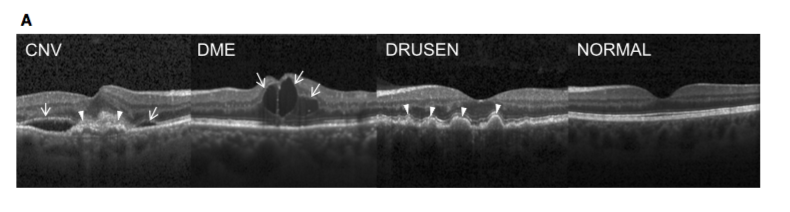
\includegraphics[width=\textwidth]{Plots/title.png}
  \caption{Beispiele für die OCT Aufnahmen der 4 Klassen.}
  \label{fig:scans}
\end{figure}
%
Es handelt sich um schwarz-weiße Bilder unterschiedlicher Größen. Die hier
gezeigten Bilder stellen ideale Beispiele der einzelnen Klassen dar.
Bei der Betrachtung des Datensatzes fällt auf, dass die Ausrichtungen der
einzelnen Bilder teilweise stark variieren. Um eine problemfreie
Verarbeitung der Daten zu gewährleisten, werden diese daher zunächst auf eine
Größe von $400\text{px}\times400\text{px}$ vereinheitlicht. Dies bedeutet also
je nach Ausgangsbild den Verlust oder das Auffüllen von Pixeln. Die Grauwerte
der Bilder werden für das Training auf einen Zahlenwert im Intervall $[0,\,1]$
skaliert.%
